\documentclass[a4paper]{article} 
\usepackage{graphicx} 
\usepackage[ngerman]{babel} 
\usepackage[ansinew]{inputenc} 
\usepackage[T1]{fontenc} 
\usepackage{tgpagella} 
\usepackage{geometry} 
\usepackage{color} 
\usepackage{microtype} 
\usepackage{minted}
\usepackage{caption}
\usepackage[headsepline,footsepline]{scrpage2}
\usepackage{textcomp}
\usepackage{pdfpages}
\usepackage{mdframed}



\makeatletter
\renewcommand\minted@pygmentize[2][\jobname.pyg]{
  \def\minted@cmd{pygmentize -l #2 -f latex -F tokenmerge
    \minted@opt{gobble} \minted@opt{texcl} \minted@opt{mathescape}
    \minted@opt{startinline} \minted@opt{funcnamehighlighting}
    \minted@opt{linenos} -P "verboptions=\minted@opt{extra}"
    -O encoding=UTF-8,outencoding=iso-8859-1 -o \jobname.out.pyg #1}
  \immediate\write18{\minted@cmd}
  % For debugging, uncomment:
  %\immediate\typeout{\minted@cmd}
  \ifthenelse{\equal{\minted@opt@bgcolor}{}}
   {}
   {\begin{minted@colorbg}{\minted@opt@bgcolor}}
  \input{\jobname.out.pyg}
  \ifthenelse{\equal{\minted@opt@bgcolor}{}}
   {}
   {\end{minted@colorbg}}
  \DeleteFile{\jobname.out.pyg}}
\makeatother


\title{Dokumentation - 6 Übung}
\author{Roman Lumetsberger}
\date{\today}

\newmintedfile[ccode]{cpp}{
               linenos,
               numbersep=5pt,
               frame=lines,
               framesep=2mm
}

\newmintedfile[javacode]{java}{
               linenos,
               numbersep=5pt,
               frame=lines,
               tabsize=2,
               framesep=2mm,
}
\newmintedfile[csscode]{css}{
               linenos,
               numbersep=5pt,
               frame=lines,
               tabsize=2,
               framesep=2mm,
}
\newmintedfile[sqlcode]{sql}{
               linenos,
               numbersep=5pt,
               frame=lines,
               tabsize=2,
               framesep=2mm,
}
\captionsetup{
  font=footnotesize,
  justification=raggedright,
  singlelinecheck=false
}


\newcommand{\srcDir}{../Beispiel/src/at/lumetsnet/caas/}
\newcommand{\testDir}{../Beispiel/test/at/lumetsnet/caas/test/}

\definecolor{lineColor}{RGB}{151,0,0}
\pagestyle{scrheadings}
\clearscrheadfoot
\begin{document}
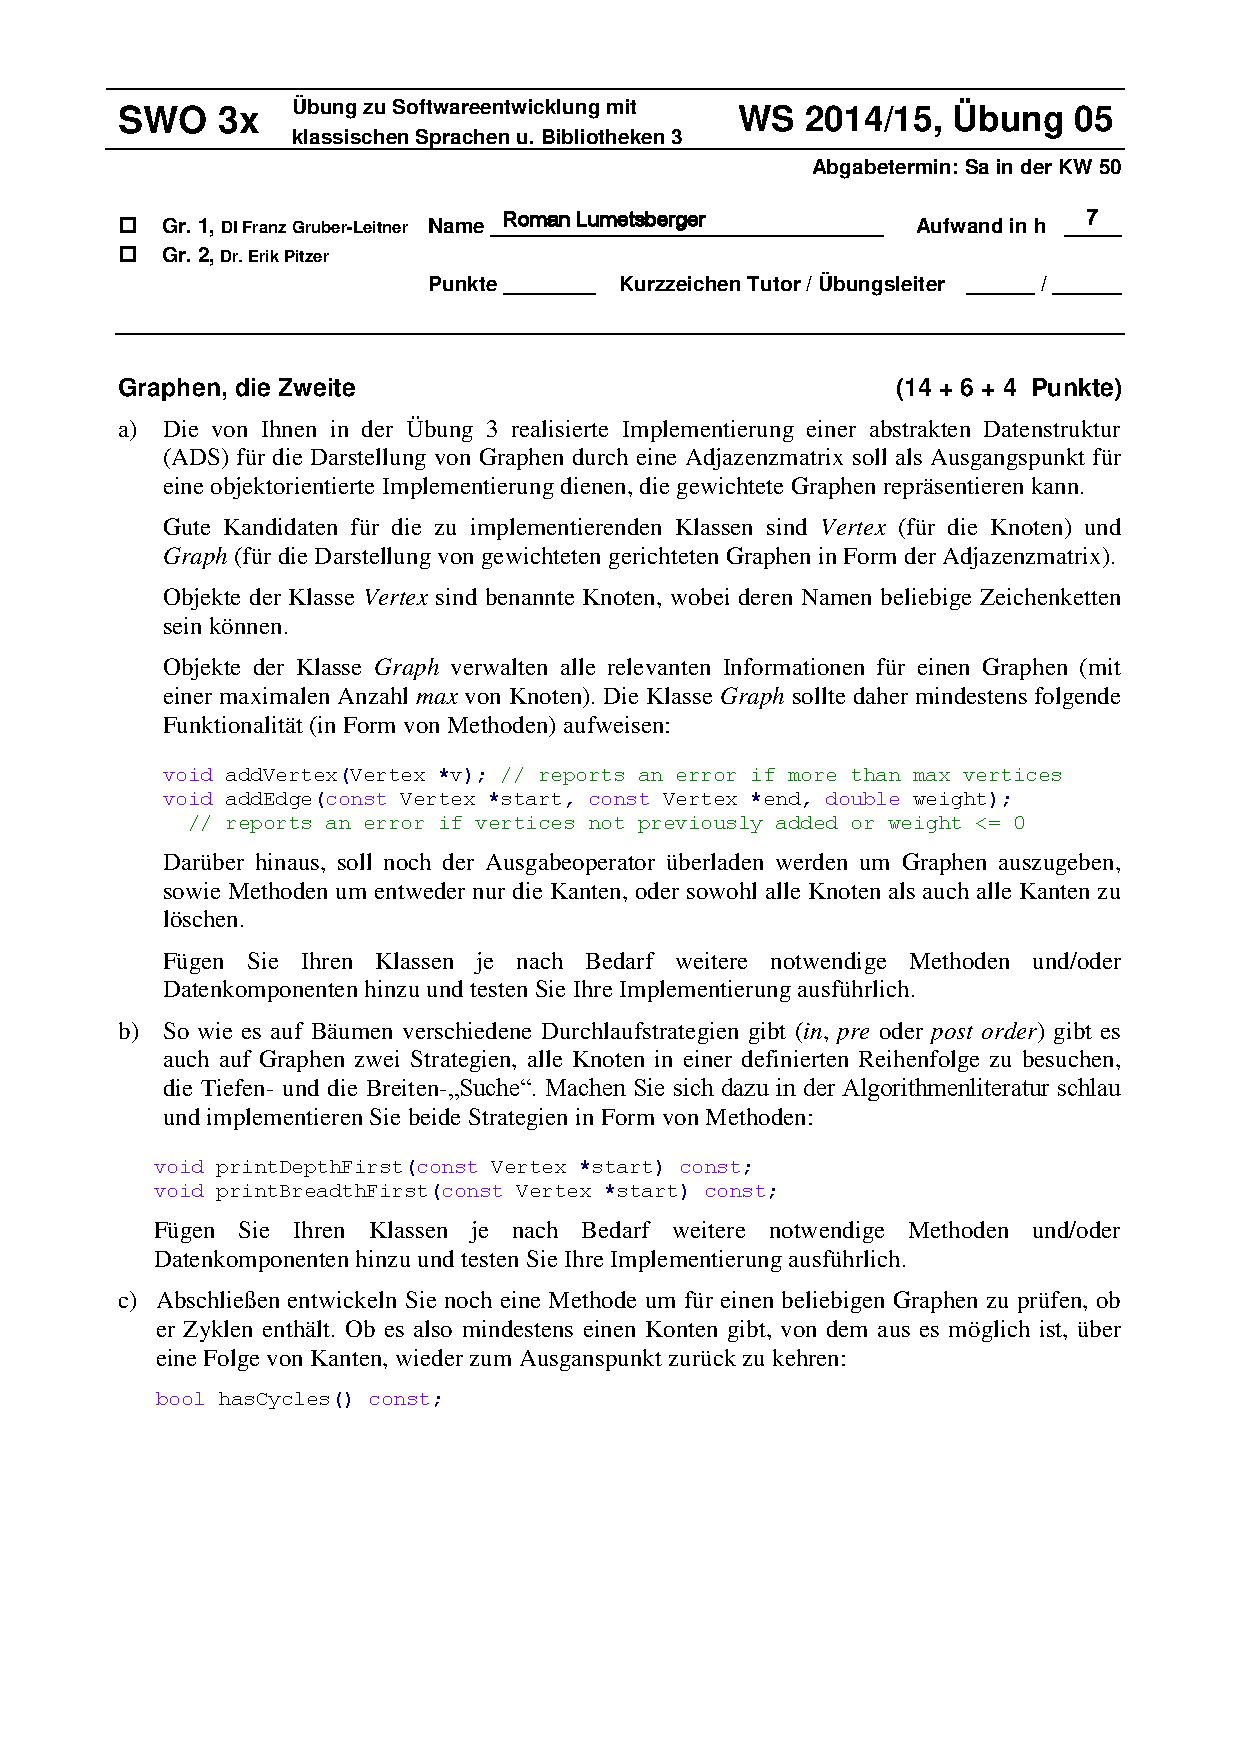
\includepdf[pages=-]{angabe.pdf}

\ihead{SWO3 WS 2014/15 - �bung 05}
\ifoot{Roman Lumetsberger}
\cfoot{1310307026}
\ofoot{Seite \pagemark}

\section{Aufgabe 1 - Graph - Objektorientiert }
\subsection{L�sungsidee}
\subsubsection{Klasse Vertex}
Es wird eine Klasse \textit{Vertex} ben�tigt, die als Datenkapsel f�r den Kontennamen ( \textit{string} ) dient.\newline
Weiters wird der Gleichheitsoperator und der Ausgabeoperator ben�tigt.

\subsubsection{Klasse Graph}
Diese Klasse enth�lt die Adjazenzmatrix und ein Array mit den Konten ( \textit{Vertex} ) des Graphen.\newline
\begin{itemize}
	\item Beim Konstruktor wird die Matrix und das Array der Knoten allokiert.
	\item Beim Hinzuf�gen von Knoten wird in das Array der Konten eingef�gt.
	\item Beim Hinzuf�gen von Kanten wird das Gewicht in die Matrix eingetragen.
	\item Beim L�schen der Kanten wird die Matrix wieder auf 0 gesetzt.
	\item Beim L�schen der Knoten wird die Matrix auf 0 gesetzt und alle Array-Elemente der Knoten auf \textit{nullptr} gesetzt.
	\item Im Destruktor wird die Matrix und das Array wieder gel�scht.
\end{itemize}	

\section{Aufgabe 2 - Graph - Durchlaufstrategien }
\subsection{Tiefensuche}
Die Tiefensuche arbeitet sich zuerst bis in die tiefste Ebene vor und besucht danach die Knoten von abzweigenden Pfaden.\newline
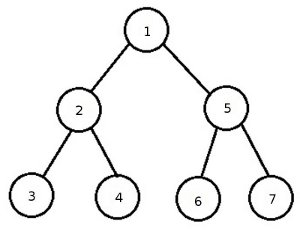
\includegraphics[width=150px]{tiefensuche.jpg}\newline

\subsubsection{Algorithmus}
Dazu wird ein Stack ben�tigt, dieser wird als eigene Hilfsklasse \textit{VertexStack} implementiert.\newline
\begin{enumerate}
	\item Das Startelement wird auf den Stack gelegt und als \textbf{besucht} markiert.
	\item Solange der Stack nicht leer ist, wird das oberste Element des Stacks betrachtet (\textit{peek}) und die n�chste Kante gesucht.
	\item
		\begin{itemize}
			\item a) Wird eine Kante zu einem Knoten gefunden, der noch nicht besucht wurde, wird dieser als \textbf{besucht} markiert und auf den Stack gelegt (\textit{push}).
			\item b) Wird keine weitere Kante gefunden, wird das Element vom Stack entfernt (\textit{pop}).
		\end{itemize}
\end{enumerate}

\subsection{Breitensuche}
Die Breitensuche besucht zuerst alle vom Startpunkt ausgehenden Knoten und arbeitet sich danach zu den tieferen Ebenen durch.\newline
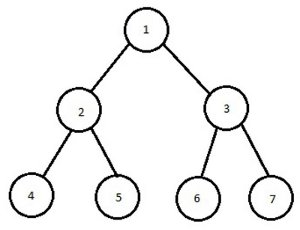
\includegraphics[width=150px]{breitensuche.jpg}\newline
\subsubsection{Algorithmus}
Dazu wird eine Queue ben�tigt, diese wird als eigene Hilfsklasse \textit{VertexQueue} implementiert.\newline
\begin{enumerate}
	\item Das Startelement wird als \textbf{besucht} markiert und alle erreichbaren Knoten in die Queue eingef�gt (\textit{enqueue}) und ebenfalls als \textbf{besucht} markiert.
	\item Solange die Queue nicht leer, ist wird das n�chste Element aus der Queue entfernt (\textit{dequeue}) und die n�chste Kante gesucht.
	\item Wird eine Kante zu einem Knoten, der noch nicht besucht wurde, gefunden, wird dieser als \textbf{besucht} markiert und in die Queue eingef�gt (\textit{enqueue}).
\end{enumerate}

\section{Aufgabe 3 - Graph - Zyklen }
Um Zyklen in einem Graphen zu erkennen, kann der Algorithmus der Tiefensuche verwendet werden und falls es eine Kante zu einem Knoten gibt, der sich bereits im Stack befindet, dann wurde ein Zyklus gefunden.
Dieses Verfahren muss f�r jeden Knoten als Startknoten wiederholt werden, falls noch kein Zyklus gefunden wurde.

\pagebreak
\subsection{Sourcecode}
\textbf{Vertex.h}
\ccode{../Beispiel/include/Vertex.h}
\textbf{VertexList.h}
\ccode{../Beispiel/include/VertexList.h}
\textbf{VertexQueue.h}
\ccode{../Beispiel/include/VertexQueue.h}
\textbf{VertexStack.h}
\ccode{../Beispiel/include/VertexStack.h}
\textbf{Graph.h}
\ccode{../Beispiel/include/Graph.h}
\textbf{Vertex.cpp}
\ccode{../Beispiel/src/Vertex.cpp}
\textbf{VertexQueue.cpp}
\ccode{../Beispiel/src/VertexQueue.cpp}
\textbf{VertexStack.cpp}
\ccode{../Beispiel/src/VertexStack.cpp}
\textbf{Graph.cpp}
\ccode{../Beispiel/src/Graph.cpp}
\textbf{main.cpp}
\ccode{../Beispiel/main.cpp}

\subsection{Testf�lle}
\subsubsection{Testfall 1 - Leerer Graph}
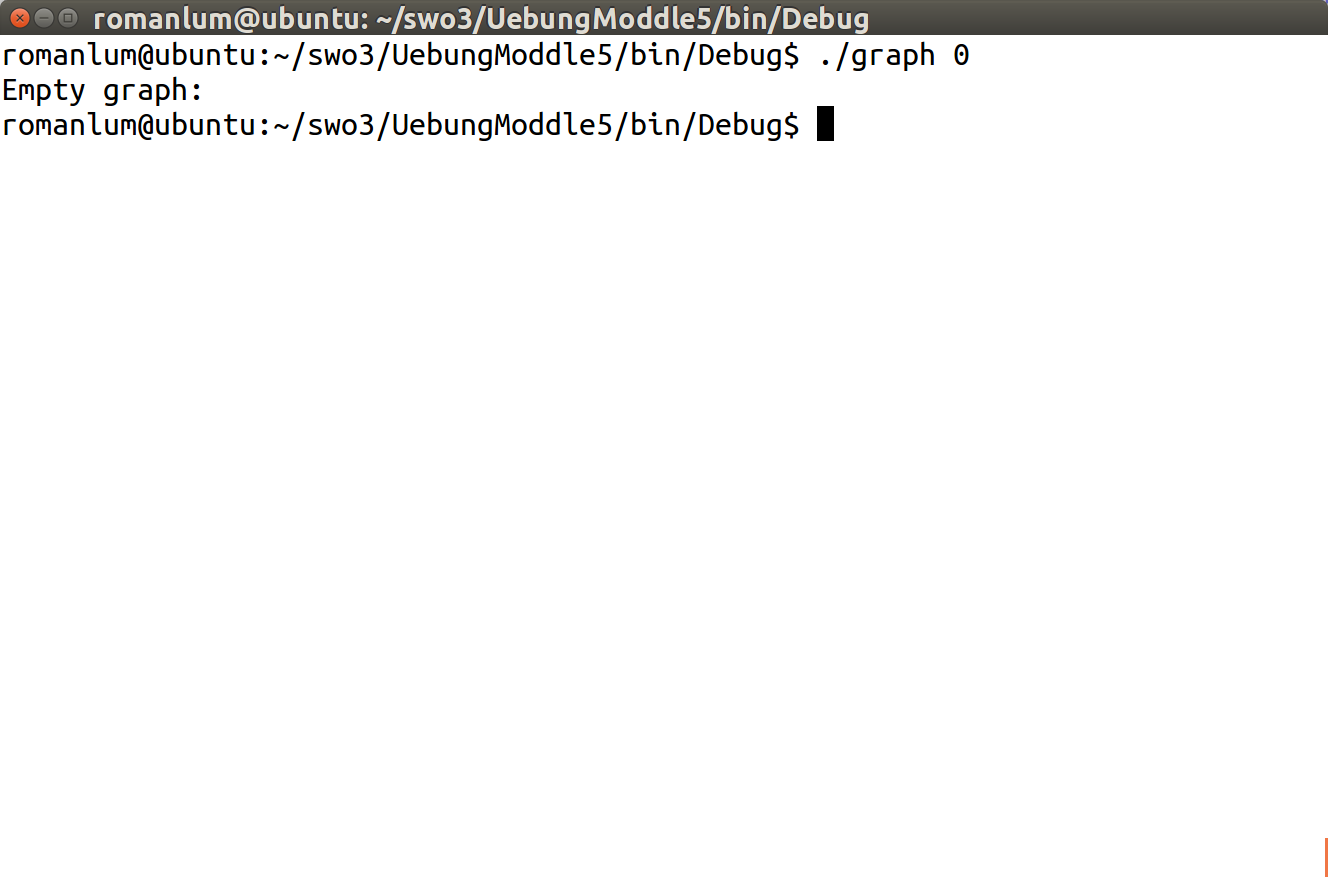
\includegraphics[width=400px, clip=true,trim=0px 600px 0px 0px]{../screenshots/0.png}
\subsubsection{Testfall 2 - Graph ohne Kanten}
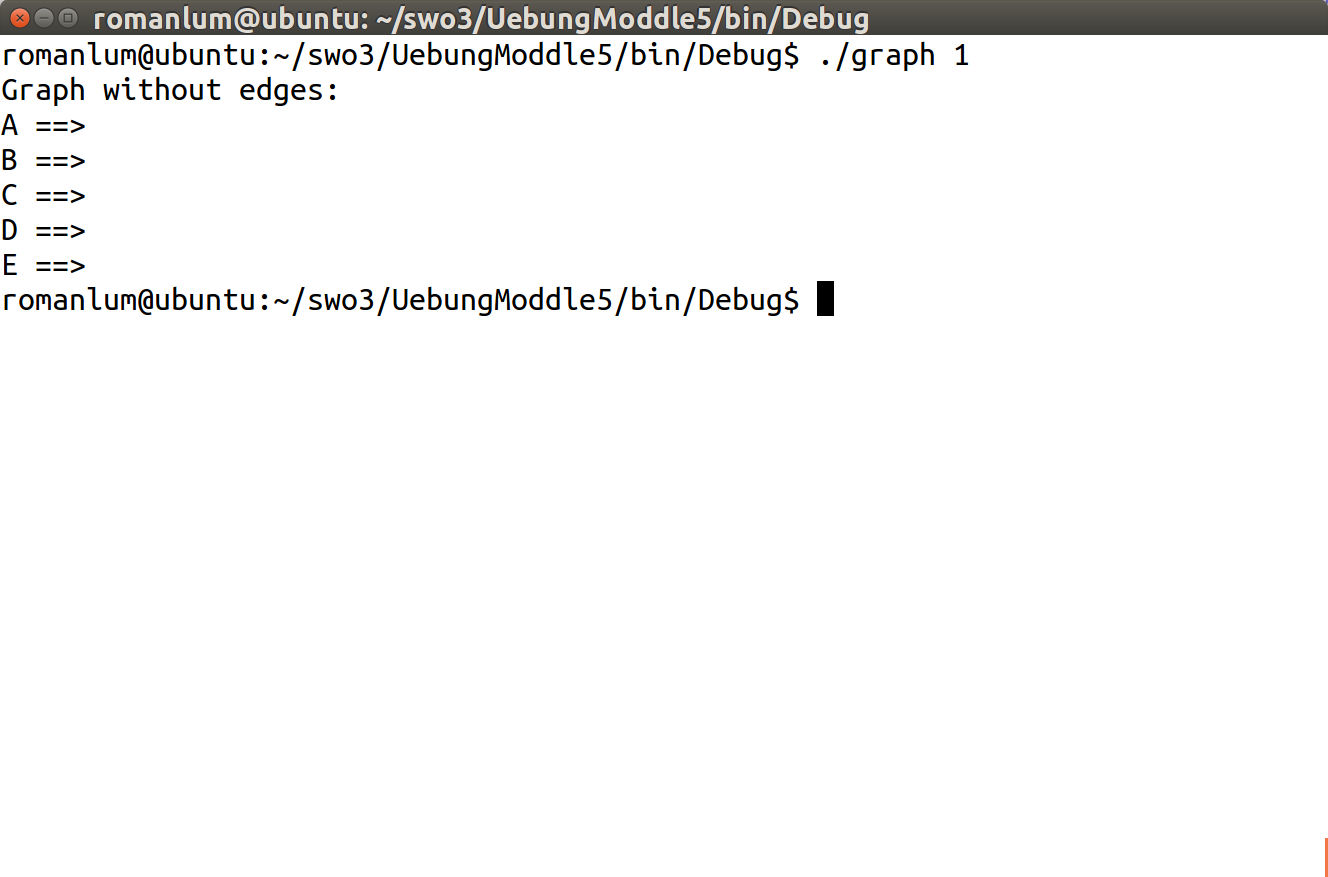
\includegraphics[width=400px, clip=true,trim=0px 500px 0px 0px]{../screenshots/1.png}
\subsubsection{Testfall 3 - Max Knotenanzahl �berschritten} 
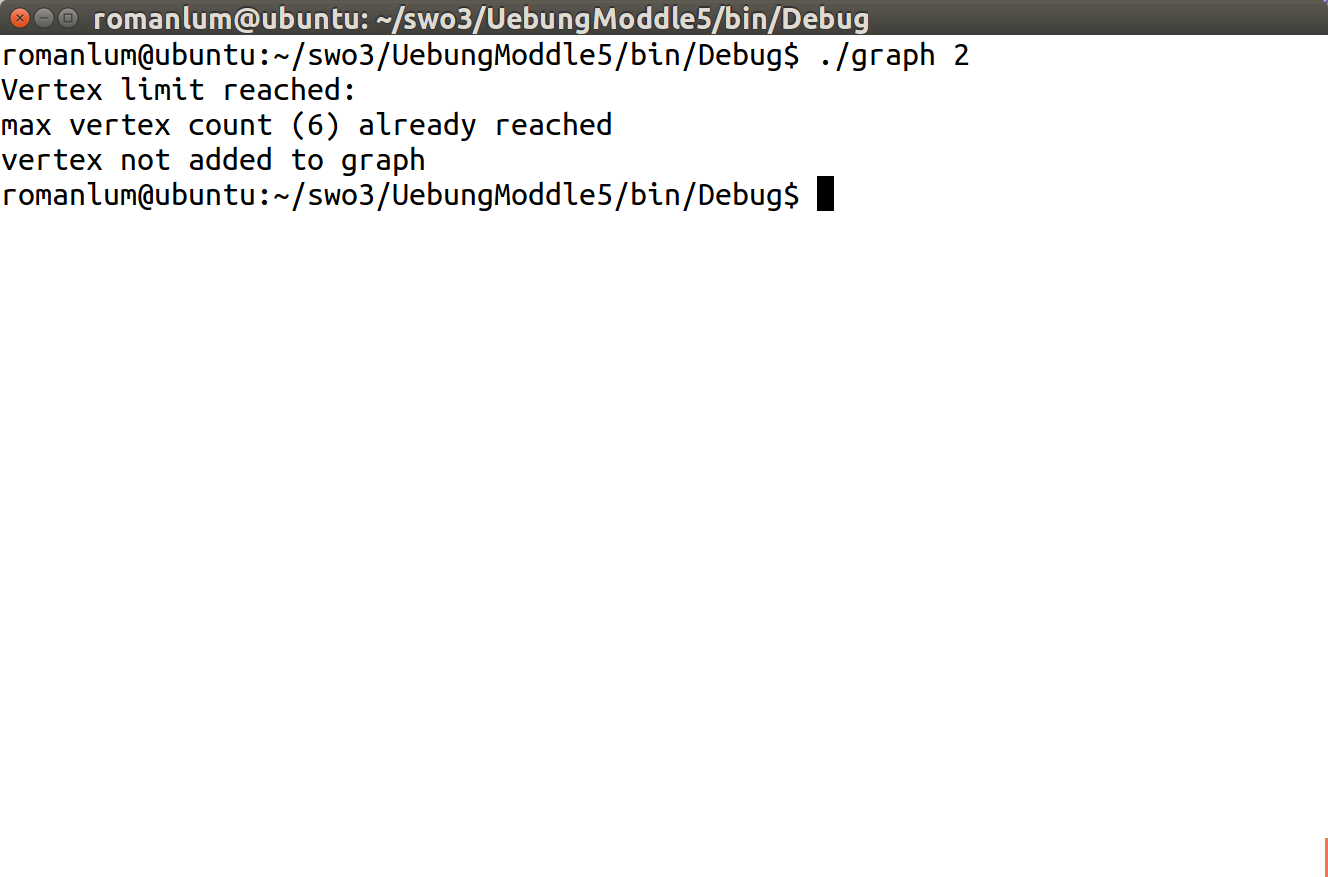
\includegraphics[width=400px, clip=true,trim=0px 600px 0px 0px]{../screenshots/2.png}
\subsubsection{Testfall 4 - Graph mit Kanten}
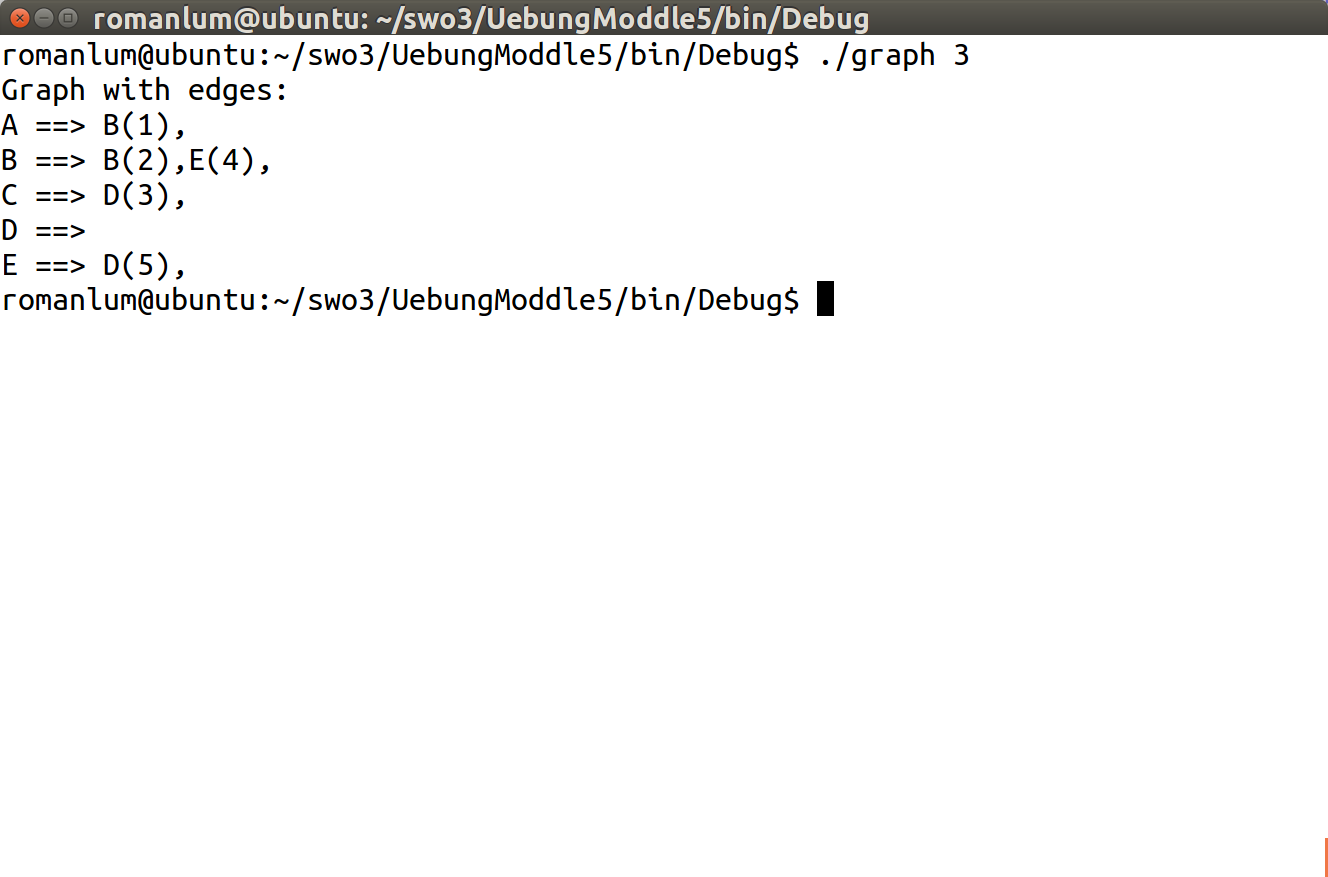
\includegraphics[width=400px, clip=true,trim=0px 500px 0px 0px]{../screenshots/3.png}
\subsubsection{Testfall 5 - Ung�ltiger Knoten / Gewicht}

\includegraphics[width=400px, clip=true,trim=0px 600px 0px 0px]{../screenshots/4.png}
\subsubsection{Testfall 6 - Kanten l�schen}
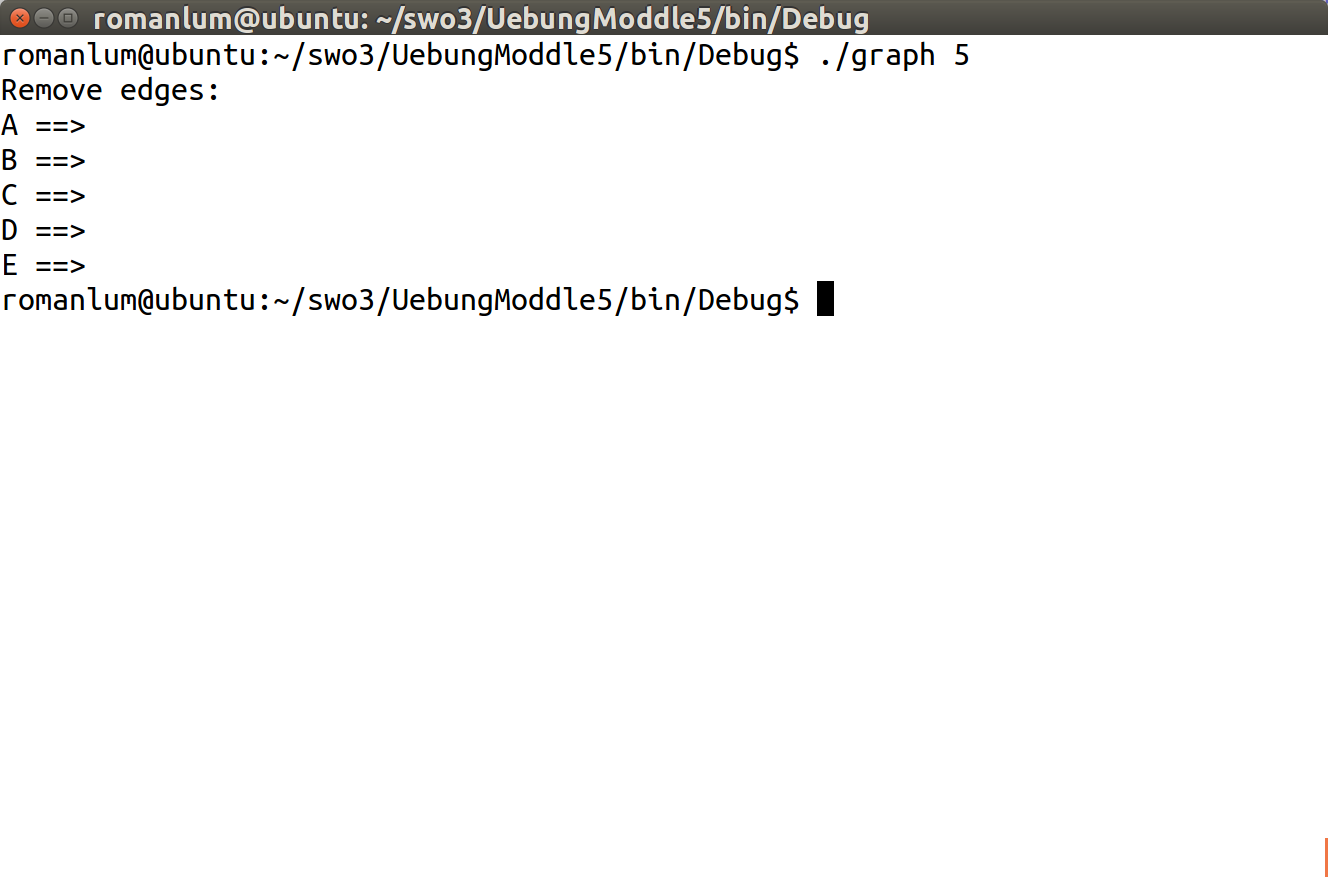
\includegraphics[width=400px, clip=true,trim=0px 500px 0px 0px]{../screenshots/5.png}
\subsubsection{Testfall 7 - Knoten l�schen / Kopierkonstruktor}
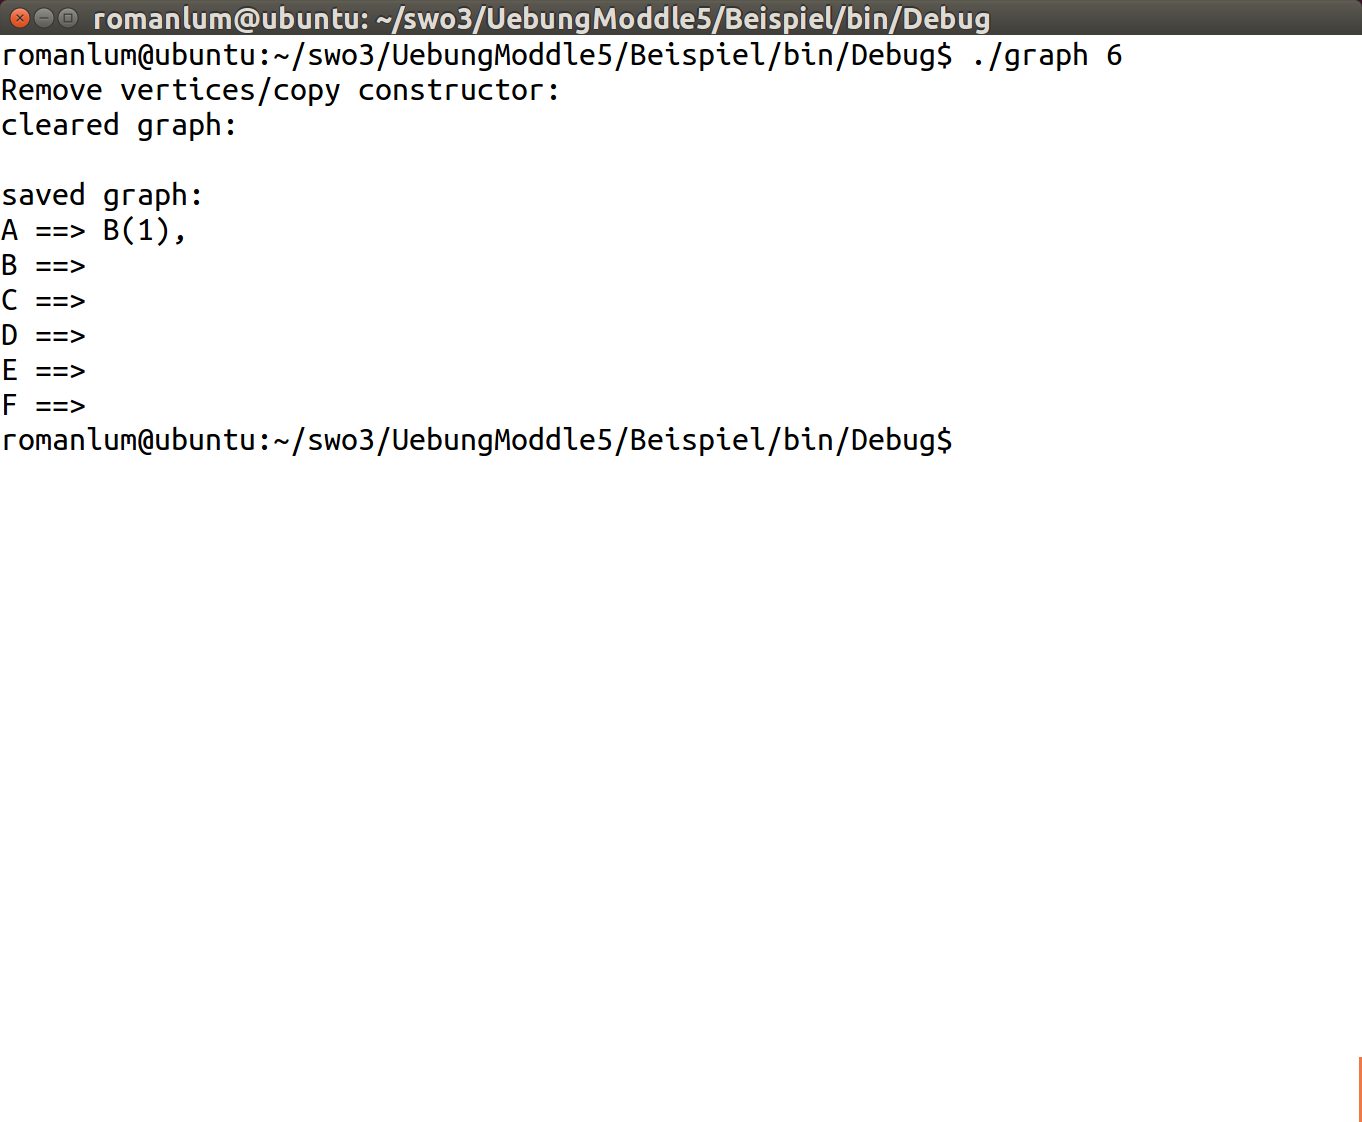
\includegraphics[width=400px, clip=true,trim=0px 600px 0px 0px]{../screenshots/6.png}
\subsubsection{Testfall 8 - Tiefensuche}
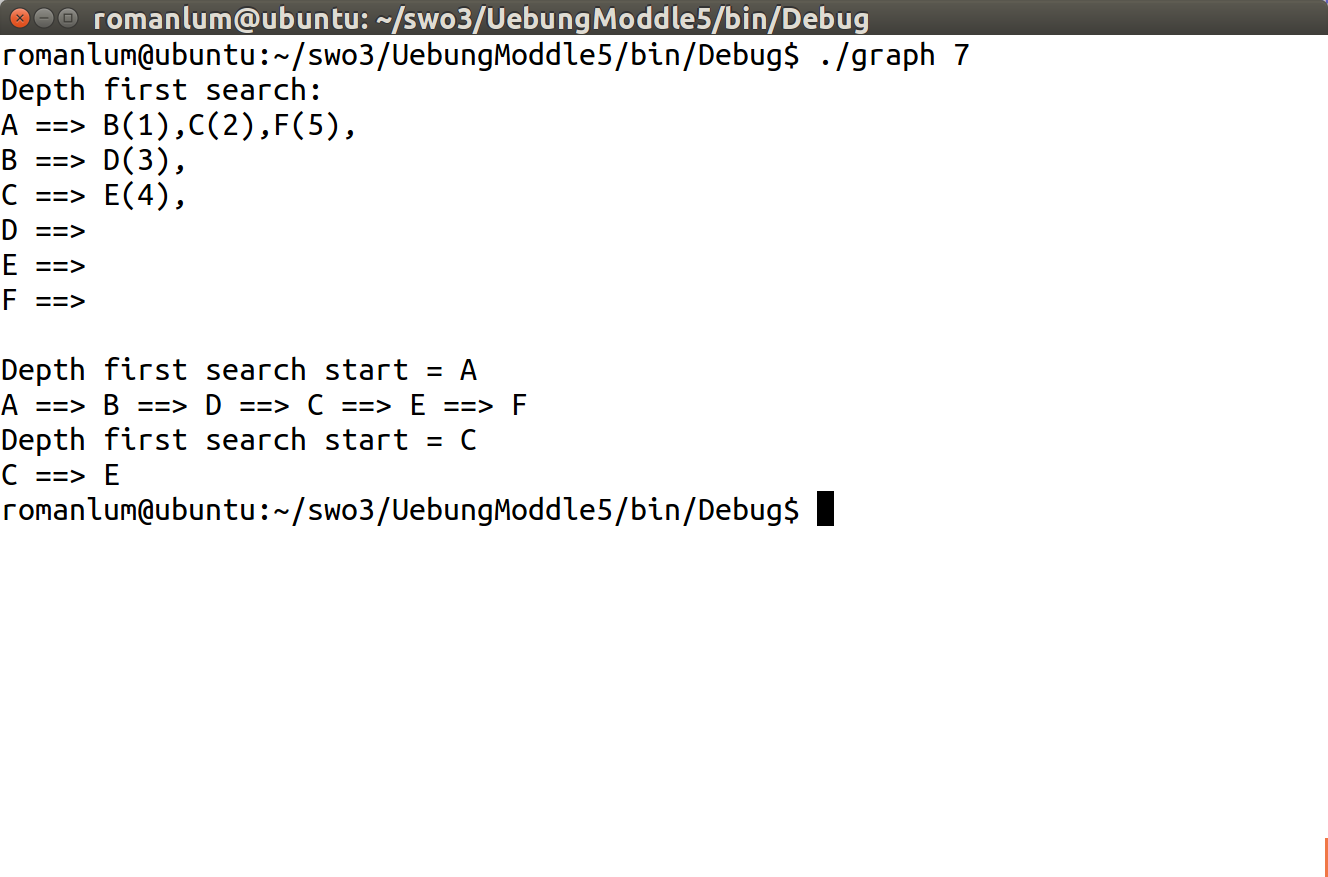
\includegraphics[width=400px, clip=true,trim=0px 200px 0px 0px]{../screenshots/7.png}
\subsubsection{Testfall 9 - Breitensuche}
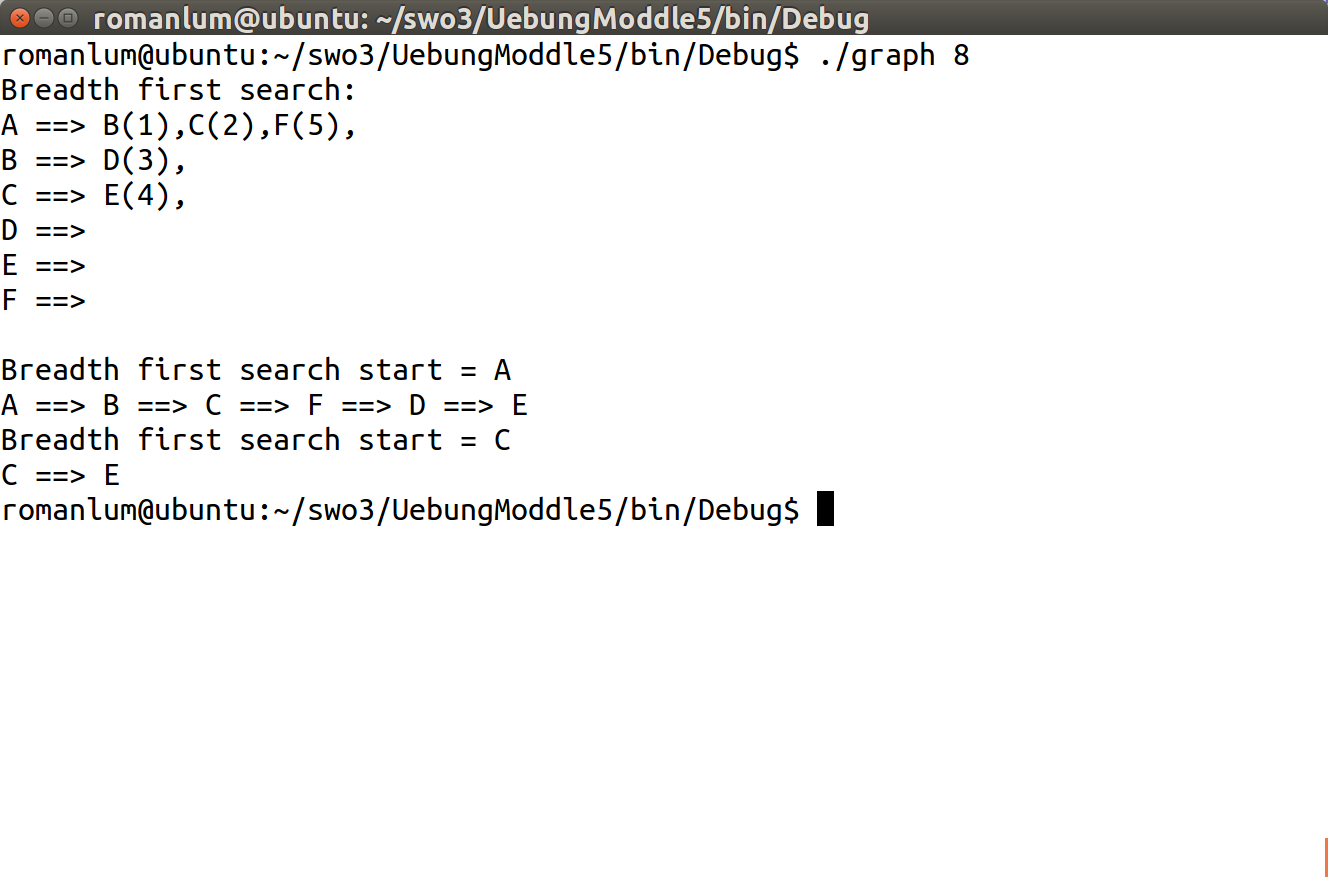
\includegraphics[width=400px, clip=true,trim=0px 200px 0px 0px]{../screenshots/8.png}
\subsubsection{Testfall 10 - Zyklen}

\includegraphics[width=400px, clip=true,trim=0px 400px 0px 0px]{../screenshots/9.png}
\subsubsection{Testfall 11 - Zyklen II}
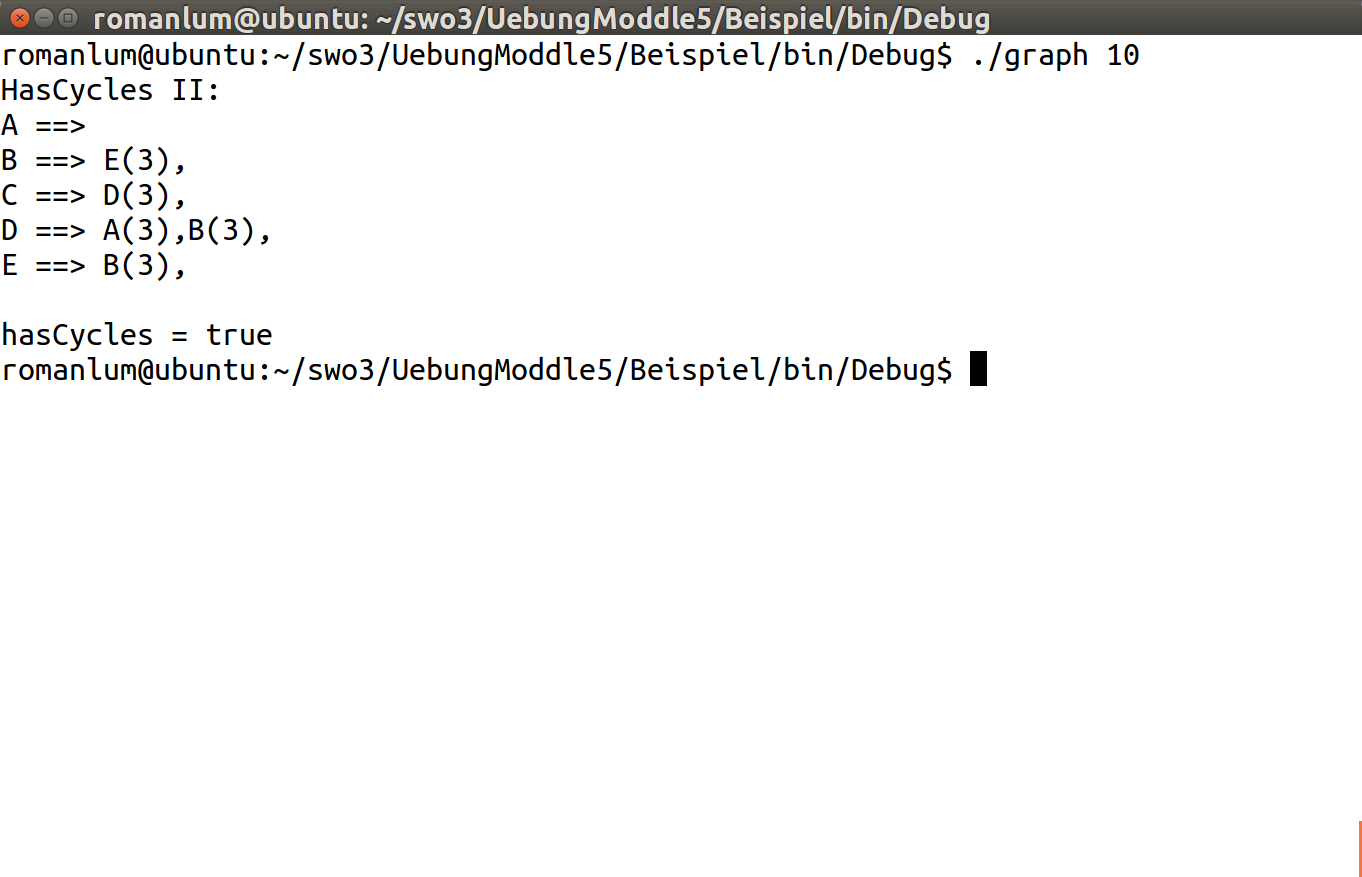
\includegraphics[width=400px, clip=true,trim=0px 400px 0px 0px]{../screenshots/10.png}
\subsubsection{Testfall 12 - Keine Zyklen}
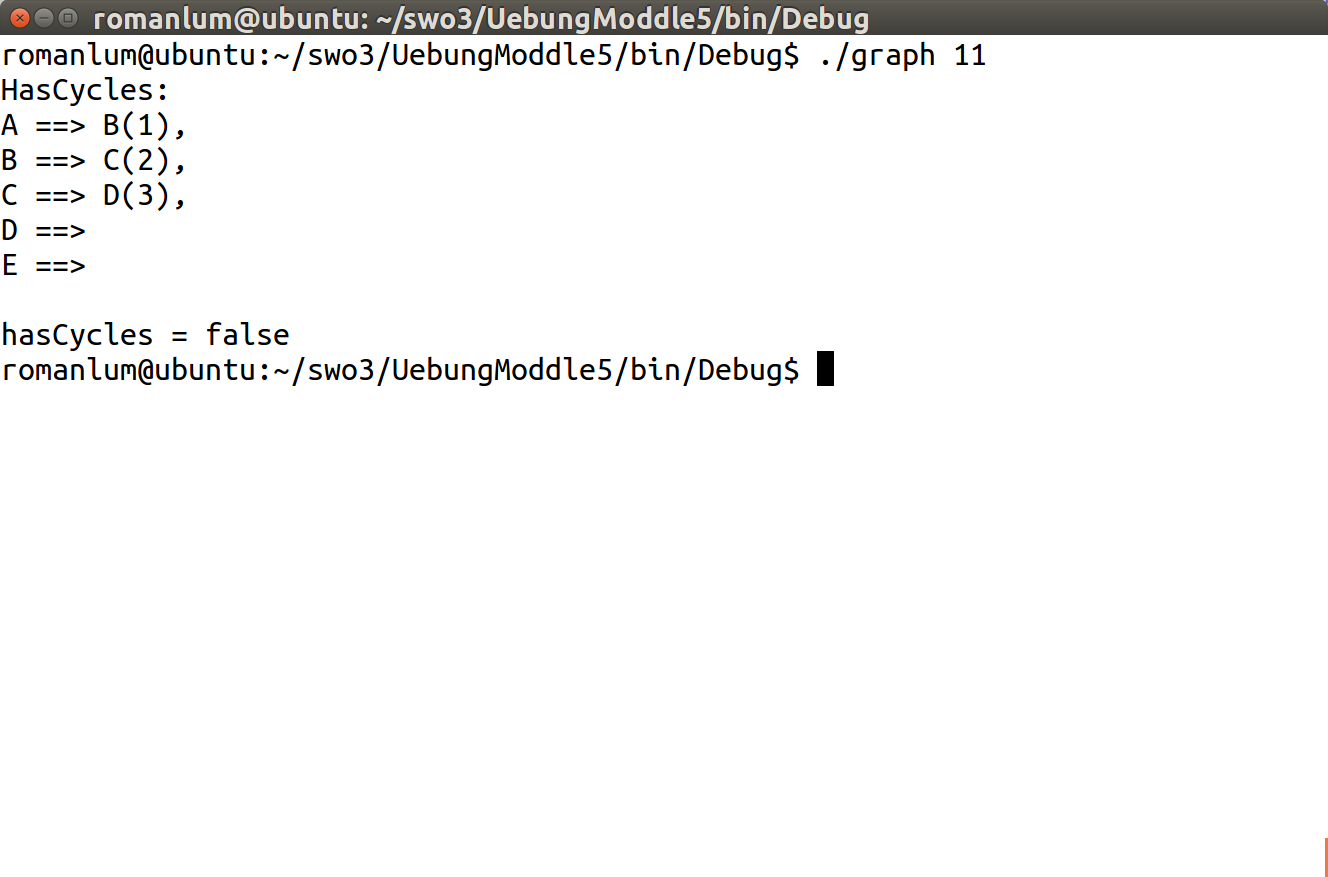
\includegraphics[width=400px, clip=true,trim=0px 400px 0px 0px]{../screenshots/11.png}
\subsubsection{Testfall 13 - Zuweisungsoperator}
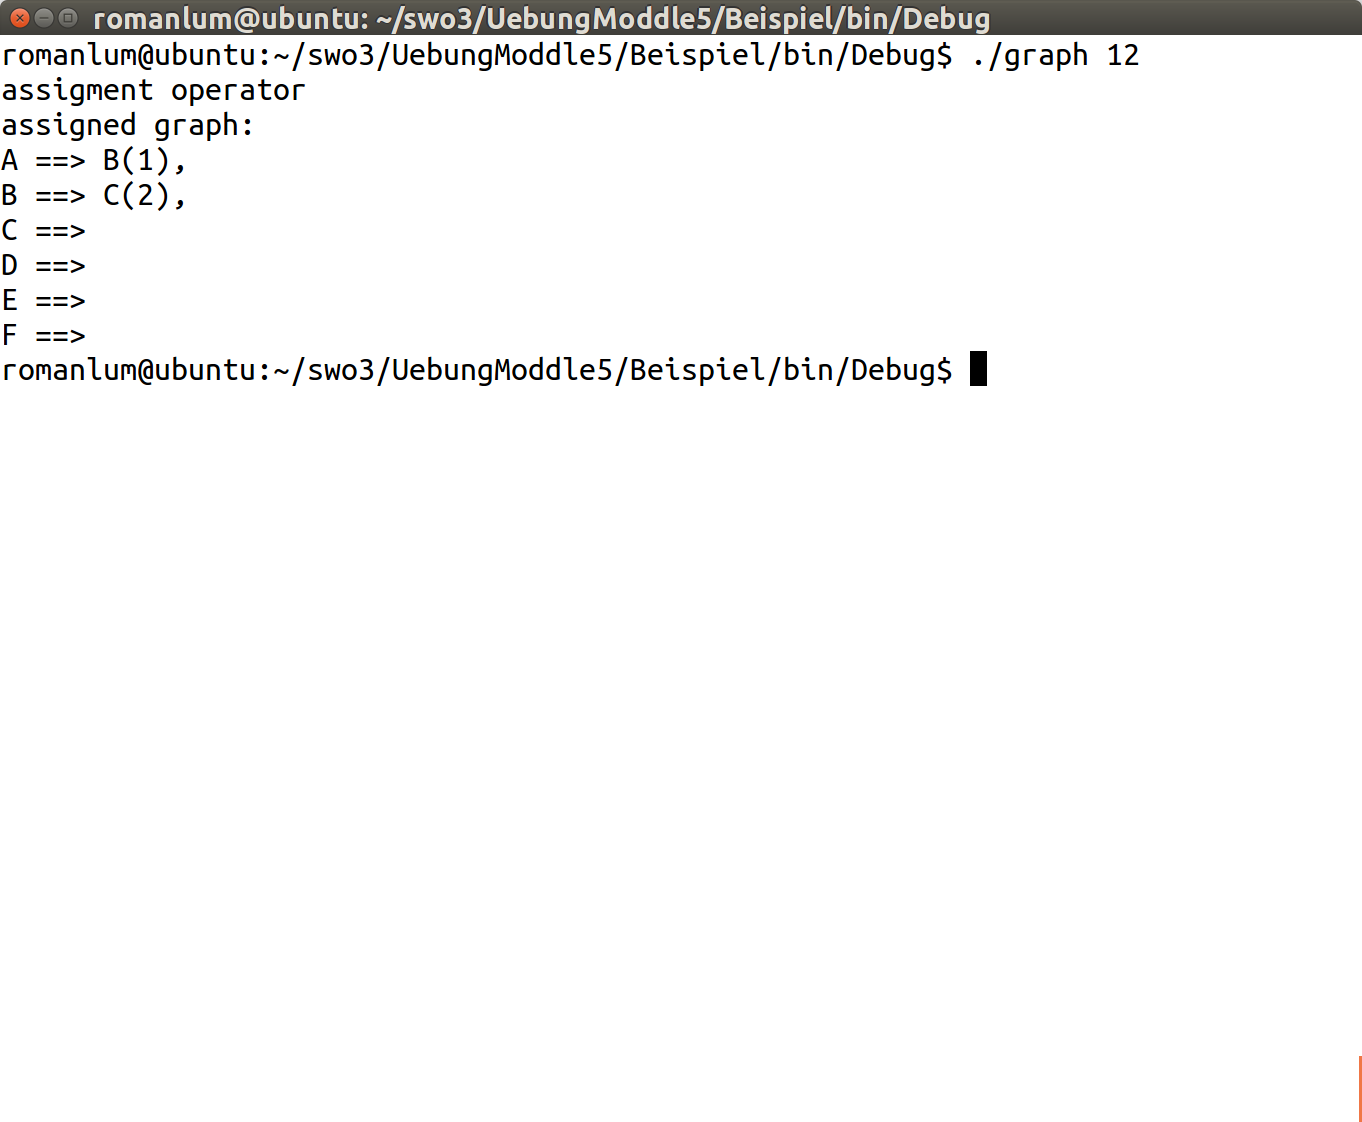
\includegraphics[width=400px, clip=true,trim=0px 000px 0px 0px]{../screenshots/12.png}
\subsubsection{Testfall 14 - Speichertest}
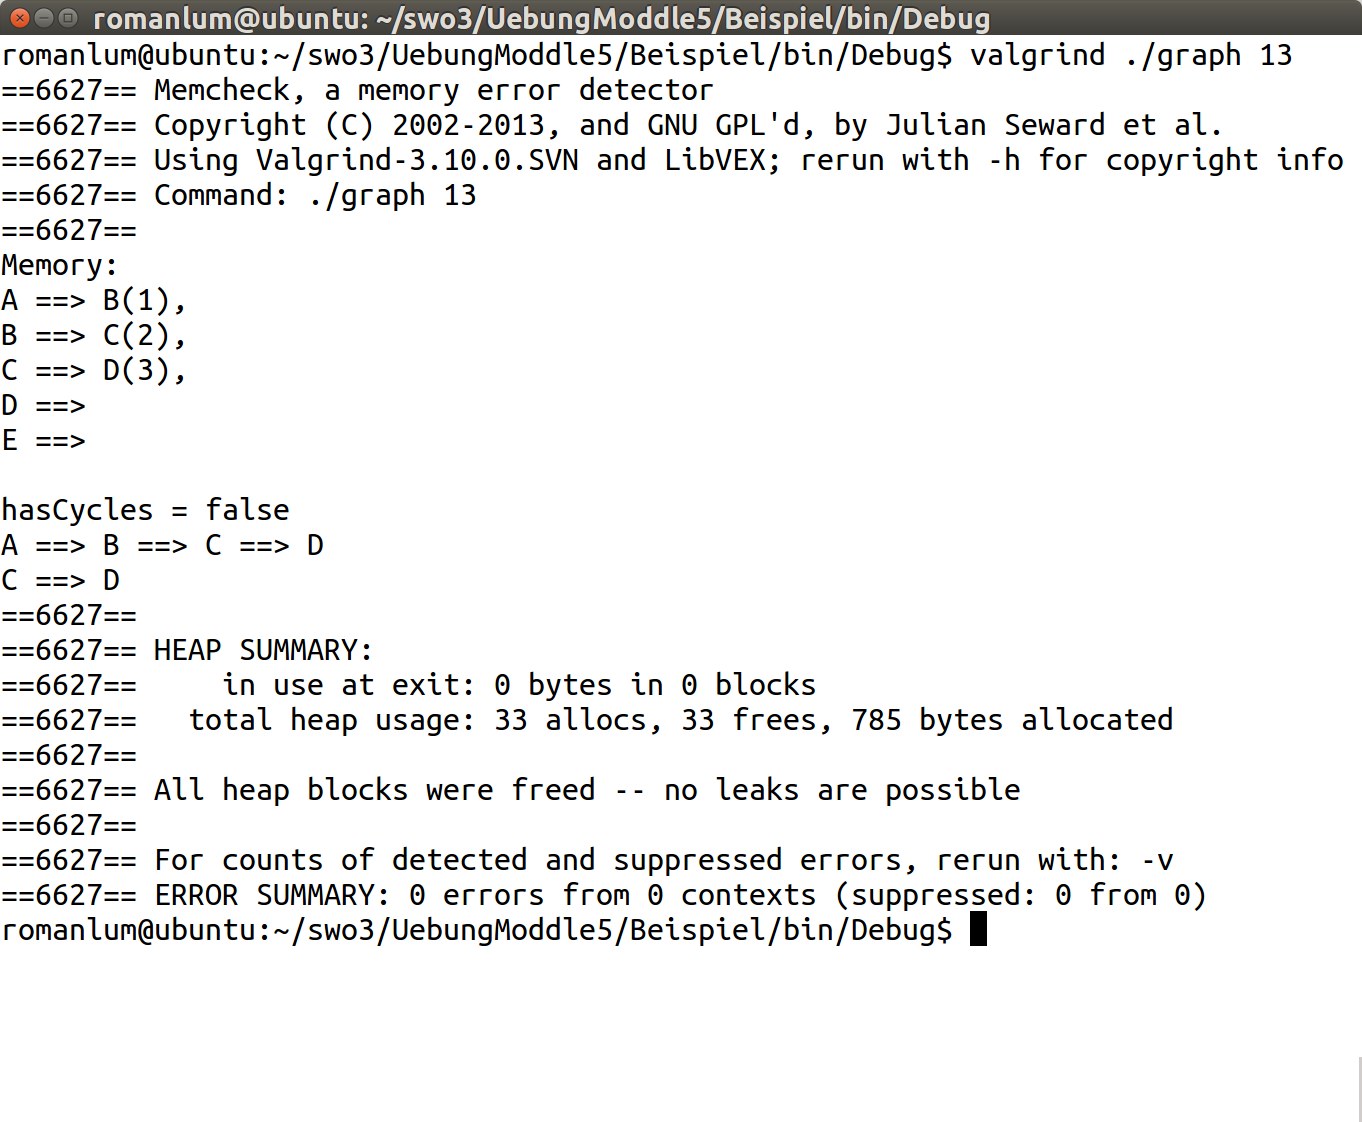
\includegraphics[width=400px, clip=true,trim=0px 000px 0px 0px]{../screenshots/13.png}


\end{document}